% !TEX root = IROS2019_DNN.tex

\begin{section}{System Models} \label{sec:model}
In this section we are going to explain the dynamic model of a quadrotor UAV and the controller model; then we are going to define the overall system as a hybrid system.

\subsection{Quadrotor UAV Dynamical Model}
A quadrotor can be modeled using the following $12^\text{{th}}$ order state vector:
\begin{equation*}
\bm{x} = \begin{bmatrix}\bm{p}_q^{\mathsf{T}} & \phi & \theta & \psi & v_x & v_y & v_z & \omega_{x} & \omega_{y} & \omega_{z}\end{bmatrix}^{\mathsf{T}}
\end{equation*}
where $\bm{p}_q=[x \; y \; z]^{\mathsf{T}}$ is the world frame position, $v_{x}$, $v_{y}$ and $v_z$ are the world frame velocities, $\phi$, $\theta$ and $\psi$ are the roll, pitch and yaw Euler angles and $\omega_{x}$, $\omega_{y}$ and $\omega_{z}$ are the body frame angular velocities \cite{BezzoAHS17, BezzoIROS2016}. The quadrotor has nonlinear dynamics: $ \dot{\boldsymbol{x}} = f(\boldsymbol{x}, \boldsymbol{u}, \boldsymbol{d}) $ where $ \boldsymbol{u} =  \begin{bmatrix} u_1 & u_2 & u_3 & u_4 \end{bmatrix} = \begin{bmatrix} F & M_1 & M_2 & M_3 \end{bmatrix} $ is the thrust and moment inputs, and $ \boldsymbol{d} = \begin{bmatrix} d_x & d_y & d_z \end{bmatrix} $ is the external disturbance. The dynamics can be described as:
\begin{equation*}
	\begin{aligned}
	\begin{bmatrix}\dot{x} & \dot{y} & \dot{z}\end{bmatrix} &= \begin{bmatrix}v_x & v_y & v_z\end{bmatrix}\\
	\begin{bmatrix}\dot{v}_x \\ \dot{v}_y \\ \dot{v}_z\end{bmatrix} &= \begin{bmatrix}0 \\ 0 \\ -g \end{bmatrix} + k_d \begin{bmatrix}d_x-v_x \\ d_y-v_y \\ d_z-v_z \end{bmatrix} \\ & + \frac{1}{m} \begin{bmatrix}\cos\phi \cos\psi \sin\theta + \sin\phi \sin\psi \\ \cos\phi \sin\theta \sin\psi - \cos\psi \sin\phi \\ \cos\theta \cos\phi \end{bmatrix} u_1 \\
	\begin{bmatrix}\dot{\phi} \\ \dot{\theta} \\ \dot{\psi}\end{bmatrix} &= \begin{bmatrix}1 & \sin\phi \tan\theta & \cos\phi \tan\theta\\ 0 & \cos\phi & -\sin\phi \\ 0 & \sin\phi \sec\theta & \cos\phi \sec\theta \end{bmatrix} \begin{bmatrix}\omega_{x} \\ \omega_{y} \\ \omega_{z} \end{bmatrix}\\
	\begin{bmatrix}\dot{\omega}_{x} \\ \dot{\omega}_{y} \\ \dot{\omega}_{z}\end{bmatrix} &= \begin{bmatrix}\frac{I_{yy} - I_{zz}}{I_{xx}} \omega_{y}\omega_{z}\\ \frac{I_{zz} - I_{xx}}{I_{yy}} \omega_{x}\omega_{z} \\ \frac{I_{xx} - I_{yy}}{I_{zz}} \omega_{x}\omega_{y} \end{bmatrix} +  \begin{bmatrix}\frac{1}{I_{xx}} & 0 & 0\\ 0 & \frac{1}{I_{yy}} & 0\\ 0 & 0 & \frac{1}{I_{zz}}\end{bmatrix} \begin{bmatrix}u_{2} \\ u_{3} \\ u_{4} \end{bmatrix}
	\end{aligned}
\end{equation*}
where $ m $ is the mass of the quadrotor, $ g $ is gravity, $ I_{xx}, I_{yy}, I_{zz} $ are the elements of the moment of inertia matrix.

\subsection{Controller Model}
In order to generate the thrust and moment inputs which make the system follow a desired trajectory or to reach a desired state, a cascaded set of PID controllers are used \cite{KumarRAM2010}. The inputs are generated as a function of the system state and the reference state on the trajectory: $ \boldsymbol{u} = g(\boldsymbol{x}, \boldsymbol{x}_{\tau}) $. Desired acceleration values are calculated using a position controller as follows:
\begin{equation*} 
	\begin{aligned}
		& a_{x,des} = \ddot{x}_{\tau} + K_{p,x} (x_{\tau}-x) + K_{d,x} (\dot{x}_{\tau}-\dot{x}) \\
		& a_{y,des} = \ddot{y}_{\tau} + K_{p,y} (y_{\tau}-y) + K_{d,y} (\dot{y}_{\tau}-\dot{y}) \\
		& a_{z,des} = \ddot{z}_{\tau} + K_{p,z} (z_{\tau}-z) + K_{d,z} (\dot{z}_{\tau}-\dot{z}) \\	
	\end{aligned}		
\end{equation*}
where $ K_{p,x}, K_{p,y}, K_{p,z} $ are the proportional parameters and $ K_{d,x}, K_{d,y}, K_{d,z} $ are the derivative parameters of the position controller. $ x_{\tau}, y_{\tau}, z_{\tau} $ are the reference positions, $ \dot{x}_{\tau}, \dot{y}_{\tau}, \dot{z}_{\tau} $ are the reference velocities and $ \ddot{x}_{\tau}, \ddot{y}_{\tau}, \ddot{z}_{\tau} $ are the reference accelerations. Based on the dynamics of the system, the desired roll and pitch angles to obtain desired acceleration values are calculated as follows:
\begin{equation*}
\begin{aligned}
	& \theta_{des} = (a_{x,des} \cos(\psi_{\tau}) +  a_{y,des} \sin(\psi_{\tau}))/g \\
	& \phi_{des} = (a_{x,des} \sin(\psi_{\tau}) +  a_{y,des} \cos(\psi_{\tau}))/g \\
\end{aligned}
\end{equation*}
where $ \psi_{\tau} $ and $ \psi_{\tau} $ are the reference yaw angle and angular velocity respectively and they are specified by the trajectory. The attitude controller is used to calculate the thrust and moment inputs as follows:
\begin{equation*}
	\begin{aligned}
		& u_1 = m (a_{z,des} + g) \\
		& u_2 = K_p (\psi_{\tau}-\psi) + K_d(\dot{\psi}_{\tau} - \dot{\psi}) \\
		& u_3 = K_p (\theta_{des}-\theta) + K_d(\dot{\theta}_{des} - \dot{\theta}) \\
		& u_4 = K_p (\phi_{des}-\phi) + K_d(\dot{\phi}_{des} - \dot{\phi}) \\
	\end{aligned}		
\end{equation*}
where $ K_p $ and $ K_d $ are the proportional and derivative parameters of the attitude controller.
 
 \subsection{Disturbance Model}
 \NB{let's add a disturbance model here}
 
\subsection{Hybrid System Model}
The overall the plant and the system can be defined as a hybrid system with two modes: safe ($ s = 1 $) and unsafe ($ s = 0 $) as shown in Fig.~\ref{fig:hybrid_model}. The inputs to the system is the reference trajectory, obstacle positions and the external disturbance. The hybrid system switch to unsafe mode when the distance between the vehicle and obstacles are smaller than the radius of the obstacle (i.e. collision with an obstacle). Once the system reach an unsafe mode, it always stays in that mode. 
\begin{figure}[h]
	\centering
	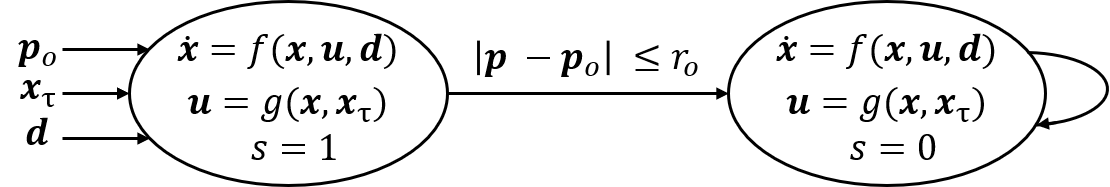
\includegraphics[width=0.4\textwidth]{figures/hybrid_system}
	\caption{Hybrid system model.}
	\label{fig:hybrid_model}
\end{figure}



\end{section}